\section{Pipelining}
As said in the previous section, pipelining comes down to splittting our circuit into subcircuits by adding registers. those registers store the informations of the previous subcircuits which makes it free to compute something else. This is that part of pipelining that makes us win a lot of time, we use the pipeline registers to free the previous part of the circuit. As said before there is a lot of backdown which makes it not perfect (see Summary (\ref{sec:summary:basicpipeline}))

\begin{parag}{Pipeline for processor}
    Pipelining is useful only if the activity in object needs to be repeated many time (as in a production line)
	\begin{itemize}
		\item We have plenty of \important{instructions} to execute
	\end{itemize}
	Pipelining needs to split the single activity in object into many subactivities
	\begin{itemize}
	\item We have a \important{good logical split} into fetch decode, execute, etc.
	\end{itemize}
	So we have already done some pipelining in lab b, all the state that we added (load1, load2, etc.) is in some way pipelining.
	
\end{parag}
\begin{parag}{A Simple multicycle CPU}
    
\end{parag}

\begin{center}
    

\begin{tikzpicture}[
    stage/.style={
        circle, draw, fill=gray!10,
        minimum size=2cm, align=center
    },
    arrow/.style={
        -{Stealth}, thick
    },
    note/.style={
        rectangle, rounded corners,
        draw=red!70!black, fill=yellow!20,
        very thick, inner sep=10pt, align=left
    }
]

% Nodes (pipeline stages)
\node[stage] (fetch) {Fetch};
\node[stage, below right=1.4cm and 1.4cm of fetch2] (decode) {Decode};
\node[stage, below left=2.8cm and 3.3cm of decode] (load) {Load};
\node[stage, left=1.4cm of decode] (alu) {ALU};
\node[stage, below left=0.6cm and 0.0cm of alu] (store) {Store};

% Arrows between stages
\draw[arrow] (fetch) edge[bend left] (decode);
\draw[arrow] (load) edge[bend left] (fetch);
\draw[arrow] (store) edge[bend left] (fetch);
\draw[arrow] (alu) edge[bend left] (fetch);
\draw[arrow] (decode) edge[bend left] node[right]{Memory} (load);
\draw[arrow] (decode)  edge[bend left] (alu);
\draw[arrow] (decode)  edge[bend left] (store);

\end{tikzpicture}
\end{center}
\begin{parag}{A Simple schedule}
	At the current moment we are doing pipelining but wihtout any pipeline registers. We are still in  sequential mode.
    \begin{center}
    \includegraphics[scale=0.2]{screenshots/2025-11-29_10.png}
    \end{center}
\end{parag}

\begin{parag}{Pipelining the processor}
    The question we want to ask now is: how far are we from acutally pipelining?\\
	We have already split our finite state machine, what we want now is to actually use those split to gain time:
	\begin{center}
	\includegraphics[scale=0.2]{screenshots/2025-11-29_11.png}
	\end{center}
	So right now we are on the left side of the images, we have every instruction that is still done sequentially. What we want is to go to the right side.
	\begin{framedremark}
	Be careful: the left one which is a \important{finite state machine}, this is not a circuit, this is an abstract representation of the working of the circuit. We will kind of mix them up (the fsm and the circuit) but they are not the same thing.
	\end{framedremark}
	So here what \texttt{F} is storing is all the information of what the cpu needs to do (reading, branching etc.), after \texttt{F} is done (fetch instruction), whatever is activated after this one is going to be put in the second block \texttt{D}. Which means that after \texttt{D} has received the information, \texttt{F} is free again of working on its own \textrightarrow compute the fetch of the next instruction
\end{parag}
\paragraph{No Hardware}%
\label{par:No Hardware}

   In a multicycle processor, some hardware components may be shared across \important{states}:
   \begin{itemize}
	   \item \important{FETCH} typically requires an \important{adder} to increment the program counter
	   \item \important{EXECUTE} naturally needs an \important{ALU}
	   \item They are \important{never used at the same time}, so the ALU can be used to increment the program counter
   \end{itemize}
   In a pipelined processor there cannot be sharing across \important{stages}, in general:
   \begin{itemize}
	   \item All stages are \important{active all the time}
	   \item Hardware needs to be \important{replicated} where appropriate
   \end{itemize}

\paragraph{Two Main Problems}%
\label{par:Two Main Problems}
\subsection{CISC vs. RISC}
	Can we \important{build equally well pipeline} for a Complex Instruction Set Computer as for a Reduced Instruction Set Computer?\\
	And what does this even means complexe, reduced?

\begin{parag}{FSM vs. Pipeline}
	If we look at any loop, at any cycle, it is an instruction, any of the path \important{represent a different instruction}. 
	\begin{itemize}
		\item \textbf{FSM}: The number of state I go from is the number of cycle I will use for each instructions.
		\item \textbf{Pipeline}: Whatever of the instruction, the instruction will have to go through all the pipeline, go through all the state.
	\end{itemize}
	
	\begin{itemize}
		\item \textbf{FSM}: \important{Any path} through the FSM represents the \important{sequence of necessary steps} for the execution of \important{an} instruction
		\item \textbf{Pipeline}: \important{The ordered path} through the pipeline is the \important{sequence of all possible steps} for the execution of \important{any} instruction
	\end{itemize}
	
	\begin{center}
	\includegraphics[scale=0.2]{screenshots/2025-11-29_12.png}
	\end{center}
    
\end{parag}
\begin{parag}{Adding an instruction to a Multi-cycle processor}
    Imagine that we only have one instruction in our multi-cycle cpu \texttt{xor} which result on the red arrow on the above image. What if we need to support the \texttt{add} instruction? To do so we wouldn't need to add any more state, the sequence of steps to execute is the same (fetch instruction, read registers, use the ALU, save result in the register), we just need to an \important{ALU that can perform additions}.
\end{parag}
\begin{parag}{Adding an instruction: not so great instruction to a Multi-cycle processor}
	Imagine now that we want to add the \texttt{lw} instruction, this time we will need a diferent path for this:
	\begin{center}
	\includegraphics[scale=0.2]{screenshots/2025-11-29_13.png}
	\end{center}
\end{parag}
\begin{parag}{Adding Instructions to a Pipeline Processor}
    So for the \texttt{xor} and \texttt{add}, the pipeline doesn't need to be changed.
\begin{center}
    

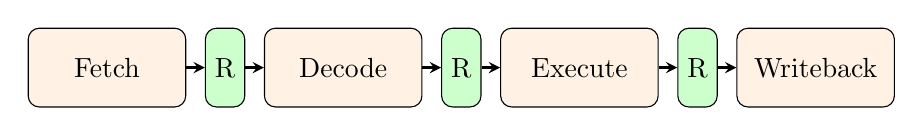
\begin{tikzpicture}[
    stage/.style={rectangle, rounded corners, minimum width=2cm, minimum height=1cm, text centered, draw=black, fill=orange!10},
    reg/.style={rectangle, rounded corners, minimum width=0.5cm, minimum height=1cm, text centered, draw=black, fill=green!20},
    arrow/.style={thick,->,>=stealth}
]


% Pipeline stages
\node[stage] (stage1) at (2,2.5) {Fetch };
\node[reg] (reg1) at (3.5,2.5) {R};
\node[stage] (stage2) at (5,2.5) {Decode};
\node[reg] (reg2) at (6.5,2.5) {R};
\node[stage] (stage3) at (8,2.5) {Execute};
\node[reg] (reg3) at (9.5,2.5) {R};
\node[stage] (stage4) at (11,2.5) {Writeback};

% Horizontal arrows for pipeline flow
\draw[arrow] (stage1.east) -- (reg1.west);
\draw[arrow] (reg1.east) -- (stage2.west);
\draw[arrow] (stage2.east) -- (reg2.west);
\draw[arrow] (reg2.east) -- (stage3.west);
\draw[arrow] (stage3.east) -- (reg3.west);
\draw[arrow] (reg3.east) -- (stage4.west);

\end{tikzpicture}

\end{center}
	But what if we wanted to add the \texttt{lw} instruction again? Then we need to add a new tube into our pipeline:
\end{parag}
\begin{center}
    
    % your TikZ code
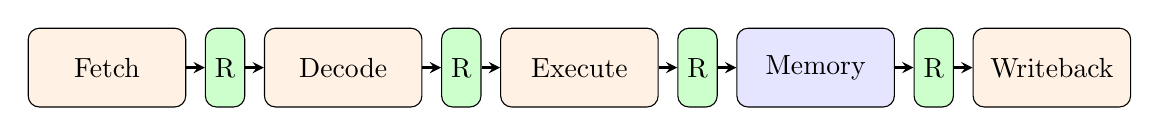
\begin{tikzpicture}[
    stage/.style={rectangle, rounded corners, minimum width=2cm, minimum height=1cm, text centered, draw=black, fill=orange!10},
    newStage/.style={rectangle, rounded corners, minimum width=2cm, minimum height=1cm, text centered, draw=black, fill=blue!10},
    reg/.style={rectangle, rounded corners, minimum width=0.5cm, minimum height=1cm, text centered, draw=black, fill=green!20},
    arrow/.style={thick,->,>=stealth}
]


% Pipeline stages
\node[stage] (stage1) at (2,2.5) {Fetch };
\node[reg] (reg1) at (3.5,2.5) {R};
\node[stage] (stage2) at (5,2.5) {Decode};
\node[reg] (reg2) at (6.5,2.5) {R};
\node[stage] (stage3) at (8,2.5) {Execute};
\node[reg] (reg3) at (9.5,2.5) {R};
\node[newStage] (stage4) at (11,2.5) {Memory};
\node[reg] (reg4) at (12.5,2.5) {R};
\node[stage] (stage5) at (14,2.5) {Writeback};

% Horizontal arrows for pipeline flow
\draw[arrow] (stage1.east) -- (reg1.west);
\draw[arrow] (reg1.east) -- (stage2.west);
\draw[arrow] (stage2.east) -- (reg2.west);
\draw[arrow] (reg2.east) -- (stage3.west);
\draw[arrow] (stage3.east) -- (reg3.west);
\draw[arrow] (reg3.east) -- (stage4.west);
\draw[arrow] (stage4.east) -- (reg4.west);
\draw[arrow] (reg4.east) -- (stage5.west);

\end{tikzpicture}

\end{center}
\begin{parag}{$ $}

	But here this is not really good, imagine that the \texttt{lw} instruction was very rarely used, we would have changed our pipeline, just to add an instruction that is used maybe 0.1\% of the time. We would have slowed our latency by one cycle for an instruction that is barely used, that doesn't seem very efficient...
	\begin{subparag}{The importance if the ISA}
	    Imagine that we want an to have an instruction (we are abusing the RISC-V syntax)
		\begin{lstlisting}[language={[RISC-V]Assembler}]
sub 8(t4), 0(t1), 0(t2)
		\end{lstlisting}
		This is a very bad instruction for us (as RISC-V programmer) but equivalent instruction exists in x86. This is a cisc instruction.\\
		But now if we go back to see how the pipeline for this instruction would look like we can see that this is horrible:\\
		\begin{center}
		\includegraphics[scale=0.2]{screenshots/2025-11-29_16.png}
		\end{center}
		This is very sad, imagine now that we try to execute the instruction \texttt{sub t4, t1, t2}
		There 6 stages that are just \important{useless}
		\begin{center}
		\includegraphics[scale=0.2]{screenshots/2025-11-29_17.png}
		\end{center}
		This is the reason for us to use \important{Reduced Instruction-Set Computer} instead of complex one.
	\end{subparag}
\end{parag}
\begin{parag}{Reduced Instruction-Set Computer}
    Instead of imposing a \important{huge penalty to every simple instruction} by making complex instruction possible, let's \important{have only similarly simple instructions} and build our programs with those.\\
	Instead of writing \texttt{sub 8(t4), 0(t1), 0(t2)} we would divide this instruction into 4 sub instruction:
	\begin{lstlisting}[language={[RISC-V]Assembler}]
lw t3, 0(t1)
lw t5, 0(t2)
sub t3, t3, t5
sw t3, 8(t4)
	\end{lstlisting}
	It turns out that is is not the only way to go, but it is a \important{good one} and we will follow it...
\end{parag}
	\begin{framedremark}
		So the only way to do pipelining efficiently is to have simple, \important{uniform instructions with similar execution paths}.
If instructions differ too much in structure or in the number of steps they require (as in CISC designs), the pipeline must include additional stages to support them, and \important{every instruction—common or rare—pays the cost} of those extra stages. This increases latency, complicates hardware, and wastes cycles.

By contrast, a Reduced Instruction-Set Computer keeps all instructions short, regular, and easy to decompose. This makes it possible to design a pipeline where \important{each stage does a small}, predictable piece of work, and all instructions flow through it smoothly. Complex operations can still be performed, but they are built from multiple simple instructions that the pipeline already supports efficiently.

In short: RISC enables clean pipelining; \important{CISC fights against it}.
That is why modern pipelined processors—and the teaching architecture we study—choose RISC-style instruction sets
	\end{framedremark}




	The question we have and that we have already seen before (see \ref{par:No Hardware}), is: What if instructions are not independent, are we able to execute code \important{correctly}?
\begin{parag}{Simple 5-Stage MIPS Pipeline}
	As an example, we wil take the first pipelined processor to be commercialized: MIP's
	\begin{center}
	\includegraphics[scale=0.2]{screenshots/2025-11-29_18.png}
	\end{center}
	\begin{framedremark}
	The reason of the \texttt{0(t2)} syntax in RISC-V. Whenever accessing or writing to memory, we always go first into \texttt{E} which is execute, which means that we actually get the addition for free here. Even if we didn't want to have that addition we would still need to go through the EXECUTE so might as well always add and add 0 when it is not needed.
	\end{framedremark}
\end{parag}
\begin{parag}{The Laundry Metaphor}
	The point here is when we have a job a sequence of things to do that you want to parallelize, some of those things are just impossible to parallelize. However in the case where parallelizing is hard to do, pipelining is very often the solution.\\
	For example, imagine we haven’t done laundry for a whole month. We would have to run about four loads. We would love to do four of them in parallel but we only have one drier, one washing machine, etc.\\
	The normal way of doing it is to launch one machine wait for it to finish. When it is done we relaunch a new load and dry the one that is clean, etc. 
	We are pipelining our clothes!
	\begin{center}
	\includegraphics[scale=0.2]{screenshots/2025-11-29_19.png}
	\end{center}
\end{parag}
\begin{parag}{Two distinct memory interfaces}
	MIPS (and most modern CPUs) usually separate \important{instruction memory} and \important{data memory}, at least logically in a pipeline. This is called the \important{Harvard architecture}. The reason for this is the following:\\
	At the FETCH stage, we read instruction from memory. In MEMORY stage we also read/write in memory. But remember what we said before (see \ref{par:No Hardware}) we cannot have two stages sharing the same circuit. This means that we need to separate them \textrightarrow instruction memory and data memory. But we cannot split our memory in two. Instead of doing two \important{distinct memories} we actually use \important{two separate caches}.
    \begin{center}
    \includegraphics[scale=0.2]{screenshots/2025-11-29_20.png}
    \end{center}
\end{parag}
\begin{parag}{What is in the Pipeline Registers}
	By definition the pipeline registers stores \important{all data that is needed later}. Every bits, ALU, wire, .. That will be used/needed later in the circuit \textbf{has to be stored} in the registers.\\
	This means that usually those are the things stored in the registers:
    \begin{center}
    \includegraphics[scale=0.2]{screenshots/2025-11-29_21.png}
    \end{center}
\end{parag}
\begin{parag}{Example of Pipelined Execution}
	For this part I won't be screenshooting 10 slides to explain the animations but you can find the explanation in the video \textit{cs-200 --4x. Instruction Level Parallelism Paolo Ienne} at 52:30.
\end{parag}
\subsection{Instruction are not independent}
All of this is nice I agree but imagine the following code:
\begin{lstlisting}[language={[RISC-V]Assembler}]
addi $r0, $r0, 1 
sub $r2, $r0, $r1
\end{lstlisting}
Now try to run this with a pipelined processor... OUCH! In the decode we need a value that is being computed in the EXECUTE, which is far away of being put in the register file.

\begin{parag}{RAW, WAR and WAW Dependences}
	\begin{subparag}{Remark}
	W is for 'write', A is for 'after' and R is for 'read'.
	\end{subparag}
	Dependency are an important thing that we will cover. Let's look at the code:
\begin{lstlisting}[language={[RISC-V]Assembler}]
divd $f0, $f1, $f2 
addd $f3, $f0, $f4
subd $f4, $f5, $f6
addi $f0, $f5, 10
\end{lstlisting}
In our code we have that:
\begin{itemize}
	\item \texttt{add} has a \important{RAW} dependence on \texttt{divd}
	\item \texttt{subd} has a \important{WAR} dependence on \texttt{addd}
	\item \texttt{adddi} has a \important{WAW} dependence on \important{divd}
\end{itemize}
The first dependence is a \important{data} dependency whereas the two other are \important{name} dependencies.\\
All of those dependencies gives us the information that those instructions has to be done sequentially, we have to wait for the other instructions to be done before starting a new one. But wait, is there really an issue with the name dependencies here? Not really, there are \textit{kind of fake}. All we have to do to make them disappear is to change the name of the registers.

As we can see the first one is way more severe that the others.
\end{parag}
\begin{parag}{Data Hazard}
	\begin{center}
	\includegraphics[scale=0.2]{screenshots/2025-11-29_22.png}
	\end{center}
	This is a \important{causality violation}. We try to use a result before it is produced.
    
\end{parag}
\begin{parag}{Data Hazards Solved by Stallig the Pipeline}
	\begin{center}
	\includegraphics[scale=0.2]{screenshots/2025-11-29_23.png}
	\end{center}
	The natural solution to \important{Data Hazards} cause by \important{RAW} dependences is to implement some logic in the processor to stop/repeat the decoding until the required value is available.

	'\important{Stalling}' roughly means introducing \texttt{nop}'s in the pipeline (we are making the code sequential again)

	Due to the rigidity of the pipeline, if one stage is stalled (\texttt{D} in the example), all the preceding ones must be stalled too (e.g., \texttt{F}).
\end{parag}
	So for us what we need to do is those two things:
	\begin{itemize}
		\item We need to understand that we have a poblem (Detecting)
		\item We have to resolve the problem  by running what is missing (Stalling)
	\end{itemize}
\begin{parag}{Detecting}
	The question we will try to answer is how do we see that we have a problem here?

	What we need to check is if the output of the EXECUTE is the same as the input at the DECODE. If they are equal then we have a problem. But this is not all, we also have to check for the other pipeline register, if any \important{pair} is detected then we have a problem.
	\begin{center}
	\includegraphics[scale=0.2]{screenshots/2025-11-29_24.png}
	\end{center}
\end{parag}
\begin{parag}{Stalling}
     We assume that we  know that there is a problem. What we need to do is to let the pipeline compute the current instruction (wihtout fetching a new one) (finish the execute). We would need a multiplexer to before the EXECUTE which would input a nop instruction instead of a rubbish instructions. After that we also need to not enable the pc and to redo the decoding of the instruction with maybe the new value.

	So here we block everything before the DECODE stage. We will block it until nobody tells me that there is an issue.
	\begin{center}
		\begin{center}
		\includegraphics[scale=0.2]{screenshots/2025-11-30.png}
		\end{center}
	\end{center}
	Now we have an example in the course which is on the course \textit{cs-200 -- 4c. Instruction Level Parallelism (cont'd)} on November 2024 at 17:00.
\end{parag}

\begin{parag}{Another Solution}
    What we were doing is adding \texttt{nop} everytime our CPU need to stall from the hardware. But adding those nop is pretty easy to detect before running the program right? so why can't you do it \important{form the software}?
	\begin{center}
	\includegraphics[scale=0.2]{screenshots/2025-11-30_1.png}
	\end{center}
	I means this doesn't look very hard to do in the software right?\\

	But is it better?\\

	Let us take here the line 3 of the left code, the \texttt{xor}. It is independent, which means that in the perspective of the stalling, it comes down to the same thing as a \texttt{nop} instruction right? So we can replace a \texttt{nop} by an independent instructions \textrightarrow we gained one instruction for \important{free}. This is a very nice compiler's problem! If we are able to build a very good compiler that is able to detect those kind of case, this means that we are able to save a pretty good amount of instructions!
\end{parag}
\begin{parag}{Architecture and Microarchitecture}
    What we are doing is \important{microarchitecure}, we are trying to opimize our CPU to do less stalls as possible.
	\begin{itemize}
		\item \textbf{Architecture}: what is in the ISA contract
			\begin{itemize}
				\item Instructions, registers, etc.
			\end{itemize}
		\item \textbf{Microarchitecture}: what is specific of an implementation
			\begin{itemize}
				\item Multi-cycle vs. pipelined, FSM or pipeline structre, etc.
			\end{itemize}
	\end{itemize}
	
	However those solutions we evoked before (reshedule instructions, add \texttt{nop}'s, delay slots) \important{expose typically microarchitectural aspects} (pipeline structure) \important{in the architecture} \textrightarrow the same binary \important{does not run} on different processor
\end{parag}
\begin{parag}{Data Hazard Solved by Forwarding Values}
    So now our pipeline works but can we make it better? For now at every stalling we loose all our progress. \\
	Let us go from the example
	\begin{center}
	\includegraphics[scale=0.2]{screenshots/2025-11-30_2.png}
	\end{center}
	So here we have a \texttt{sub} right after an \texttt{addi}. If we take our pipeline the result of our add is actually computed right after the EXECUTE stage:


\end{parag}
    

\begin{center}
    
    % your TikZ code
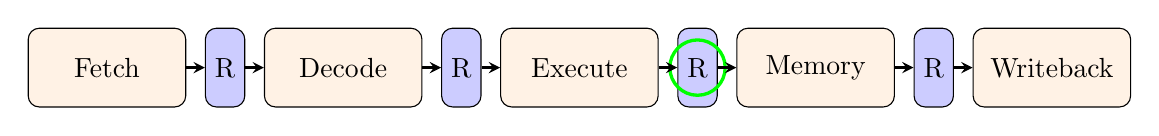
\begin{tikzpicture}[
    stage/.style={rectangle, rounded corners, minimum width=2cm, minimum height=1cm, text centered, draw=black, fill=orange!10},
    newStage/.style={rectangle, rounded corners, minimum width=2cm, minimum height=1cm, text centered, draw=black, fill=blue!10},
    reg/.style={rectangle, rounded corners, minimum width=0.5cm, minimum height=1cm, text centered, draw=black, fill=blue!20},
    arrow/.style={thick,->,>=stealth}
]


% Pipeline stages
\node[stage] (stage1) at (2,2.5) {Fetch };
\node[reg] (reg1) at (3.5,2.5) {R};
\node[stage] (stage2) at (5,2.5) {Decode};
\node[reg] (reg2) at (6.5,2.5) {R};
\node[stage] (stage3) at (8,2.5) {Execute};
\node[reg] (reg3) at (9.5,2.5) {R};
\draw[green, very thick] (9.5, 2.5) circle (10pt);
\node[stage] (stage4) at (11,2.5) {Memory};
\node[reg] (reg4) at (12.5,2.5) {R};
\node[stage] (stage5) at (14,2.5) {Writeback};

% Horizontal arrows for pipeline flow
\draw[arrow] (stage1.east) -- (reg1.west);
\draw[arrow] (reg1.east) -- (stage2.west);
\draw[arrow] (stage2.east) -- (reg2.west);
\draw[arrow] (reg2.east) -- (stage3.west);
\draw[arrow] (stage3.east) -- (reg3.west);
\draw[arrow] (reg3.east) -- (stage4.west);
\draw[arrow] (stage4.east) -- (reg4.west);
\draw[arrow] (reg4.east) -- (stage5.west);

\end{tikzpicture}

\end{center}
\begin{parag}{$ $}
    So our issue here is that we need the output of the EXECUTE at the input of the EXECUTE. Might as well create a bypasse path for this right? 
\end{parag}
\begin{center}
    
    % your TikZ code
\begin{tikzpicture}[
    stage/.style={rectangle, rounded corners, minimum width=2cm, minimum height=1cm, text centered, draw=black, fill=orange!10},
    newStage/.style={rectangle, rounded corners, minimum width=2cm, minimum height=1cm, text centered, draw=black, fill=blue!10},
    reg/.style={rectangle, rounded corners, minimum width=0.5cm, minimum height=1cm, text centered, draw=black, fill=blue!20},
    arrow/.style={thick,->,>=stealth}
]


% Pipeline stages
\node[stage] (stage1) at (2,2.5) {Fetch };
\node[reg] (reg1) at (3.5,2.5) {R};
\node[stage] (stage2) at (5,2.5) {Decode};
\node[reg] (reg2) at (6.5,2.5) {R};
\node[stage] (stage3) at (8,2.5) {Execute};
\node[reg] (reg3) at (9.5,2.5) {R};
\node[stage] (stage4) at (11,2.5) {Memory};
\node[reg] (reg4) at (12.5,2.5) {R};
\node[stage] (stage5) at (14,2.5) {Writeback};

% Horizontal arrows for pipeline flow
\draw[arrow] (stage1.east) -- (reg1.west);
\draw[arrow] (reg1.east) -- (stage2.west);
\draw[arrow] (stage2.east) -- (reg2.west);
\draw[arrow] (reg2.east) -- (stage3.west);
\draw[arrow] (stage3.east) -- (reg3.west);
\draw[arrow] (reg3.east) -- (stage4.west);
\draw[arrow] (stage4.east) -- (reg4.west);
\draw[arrow] (reg4.east) -- (stage5.west);


% Additional arrow from reg3 east to Execute west (bypass/forwarding path)
\draw[arrow, red, thick] (reg3.east) 
    to[out=0, in=0, looseness=3] 
    ($(stage3.west) + (0,0.9)$) 
    to[out=30, in=180] 
    (stage3.west);
% Label for the bypass path
\node[above, red, align=center, font=\small] at ($(reg3.east) + (0, 0.8)$) {Bypass/\\Forwarding Path};


\end{tikzpicture}

\end{center}
\begin{parag}{ $ $}
    So now we need to add a multiplexer for us two know if we need to take the forwarding path or not.

	However this is a little glitch here:
	What does those register contains? Imagine that:
	\begin{itemize}
		\item We are forwarding E \textrightarrow E (ALU result to the next ALU input)
		\item M \textrightarrow E forwarding (Data memory output or ALU result from M stage)
		\item W \textrightarrow D forwarding (register file writeback in same cycle as read)
	\end{itemize}
	Now the 'glitch' happens in the W \textrightarrow D register file forwarding. The register file must:
	\begin{itemize}
		\item \important{write} a value in W stage
		\item \important{read} it in the D stage of the next instruction
	\end{itemize}
	\begin{center}
	    \textbf{in the same clock cycle}
	\end{center}
	This is just \important{impossible}.\\
	In order to resolve this issue we have to check in the DECODE if the register that we took from is valid or not \textrightarrow we need some bits of information that tell us wether the register we are using is valid or not.\\
	Us from two pages ago would take those valid bits as redundancy, we need the \important{value} and \important{register}.\\
	We then check with a multiplexer if the register value is rubbish or is it valid. If it is rubbish we then use one of the red arrow, else the value.
\end{parag}


\begin{parag}{Classic MIPS pipeline}
    For a classic 5-stage pipeline with \important{all forwarding paths}:
	\begin{itemize}
		\item E \textrightarrow E, M \textrightarrow E
		\item W \textrightarrow D
	\end{itemize}
	The \important{register-file forwarding} (W \textrightarrow D) is a special case:
	\begin{itemize}
		\item During \textbf{W}, registers are written in the \important{first half} of the cycle
		\item During, \textbf{D}, registers are read in the \important{second half} of the cycle.
	\end{itemize}
	\begin{subparag}{How can we divide our clock cycle}
	    The way of doing it is use level sensitives, we write in our register-file when there is a rising edge of the clock, we read our register-file when there is a lower edge of the clock. The write occurs when \texttt{clk} is high, the read occurs when the \texttt{clk} is low.
	\end{subparag}
	This means that a register can be correctly written and read in the same cycle
	\begin{center}
	\includegraphics[scale=0.2]{screenshots/2025-11-30_3.png}
	\end{center}
	Example again on \textit{cs-200 4c. Instruction Level Parallelism November 20, 2024 at 1:05}
	But here we have saved a lot of stalling, our pipeline is almot perfect. The only stalling we still get is when we are decoding a register that is in E but need to be loaded for instance:
	\begin{lstlisting}[language={[RISC-V]Assembler}]
lw r9, 0(r7)
sub r3, r9, r1
	\end{lstlisting}
	So here \important{most of the stalls} are removed.
	\begin{subparag}{Remark}
	    This is only something that can be done in hardware, this is not possible to do from a software perspective.
	\end{subparag}
\end{parag}


\subsubsection{Structural Hazards}
\begin{definition}[structural hazard]
A \important{structural hazard} happens when different instructions compete for the same ressource (e.g., pipeline stage)

It is a \important{ressource conflict}.
\end{definition}
Our structural hazards \important{canot happen} in our pipeline. If we did not stall also instructions following one missing an operand, we could have structural hazards.
	\begin{center}
	\includegraphics[scale=0.25]{screenshots/2025-11-30_4.png}
	\end{center}

	But what happen if we have a \important{cache miss}? If we have a data cache miss, then we have to wait for the cache to responds, all the previous stage are stalling, the W stage on the other hand can advance (the same principle goes for the F stage).

	\begin{parag}{What about miss on both side?}
		So here if we have two miss then we have a \important{structural hazard} on main memory. The way of solving them is to let the most right miss have the priority.
	\end{parag}


\begin{parag}{Control Hazard}
	Let us take for instance this code:
    \begin{center}
    \includegraphics[scale=0.2]{screenshots/2025-11-30_5.png}
    \end{center}
	Here we have a big issue, after the branch instruction, what should we fetch? We don't know which instruction we should have fetched. This is a \important{causality violation}
\end{parag}
\begin{parag}{Control hazard solved by stalling}
    So here the easy way of solving it is to stall the pipeline when we have a branch. 
	\begin{center}
	\includegraphics[scale=0.2]{screenshots/2025-11-30_6.png}
	\end{center}
	Similarly to the way we solve data hazards, we can \important{stall the pipeline} (F), one it is discovered, after \textbf{D}, that an instruction was a branch, and this \important{until the branch is resolved}.\\

	If, for instance the correct address of the next instruction is know at the end of the E stage, \important{2 cycles are lost every branch}
\end{parag}
\begin{parag}{Fetching and decoding do not do any damage}
	Maybe we can have a slightly better view of that. After all we are not fetching rubbish in the first case. There is a possibility that the instruction that we have fetched is actually correct.
    \begin{center}
    \includegraphics[scale=0.2]{screenshots/2025-11-30_7.png}
    \end{center}
	\begin{itemize}
		\item Fetching or decoding a wrong instruction does not create any problem, provided that the instruction is not also \important{executed}
		\item If the outcome of the branch is known at the end of the E stage, we can \important{wait} until then to \important{conditionally kill} the following two instructions in the pipeline \important{if the branch happens to be taken}
		\item Now \important{2 cycles are lost only for taken branches} and \important{none is lost for nontaken ones}
	\end{itemize}
\end{parag}
\begin{parag}{Another solution}
    As we have seen for data hazard, we  can also use the software in order to resolve those hazards. We could just add \texttt{nop} at this good place which would resolve our hazard.
\end{parag}
\begin{parag}{Control Hazard Solved by Delay Slot}
	\begin{center}
	\includegraphics[scale=0.2]{screenshots/2025-11-30_8.png}
	\end{center}
	Alternatively, we can \important{modify the definition of the architecture} and decide that \important{the two instructions following a branch are executed in any case} (branch taken or not) as if they were before (same thing as in cs-328). Thse instructions after the branches are called \important{delay slots}, before when a branch happened we added \texttt{nop}, so might as well try to compute someting instead right? 
	But now our code becomes \important{counterintuitive}, we execute code maybe for nothing.
	\begin{subparag}{Remark}
	    MIPS did it as some others, but quite rare in current architectures
	\end{subparag}
\end{parag}
\begin{parag}{Use of Delay Slots}
	A simple way of using delay slots is to use them for \texttt{nop}'s-- but then it is not better than stalling the pipeline. A better idea is to put there instructions which precede the branch and on which the branch has \important{no dependence}.
	Suppose an architecture with two delay slots:
	\begin{lstlisting}[language={[RISC-V]Assembler}]
sub r2, r0, r7
mul r1, r6, r7
add r5, r3, r4 
beq r0, r1, loop 
nop
nop
lw r8, 12(r9)
	\end{lstlisting}
	Then this can be turned into:
\begin{lstlisting}[language={[RISC-V]Assembler}]
mul r1, r6, r7
beq r0, r1, loop 
sub r2, r0, r7 
add r5, r3, r4 
lw r8, 12(r9)
\end{lstlisting}
We use some instructions that is independent to fill the nop instructions
\end{parag}



\begin{parag}{Branch Prediction}
	\begin{itemize}
		\item A better strategy is to \important{guess the branch outcome} and fetch the corresponding instruction (either the next instruction or the branch destination, but not nessarily the former)
			\begin{itemize}
				\item If the guess is correct, \important{no cycle is lost}
				\item If the guess is wrong, what has been fetched and decoded is thrown away (\important{squashed})
			\end{itemize}
		\item Branch predictors of modern processors are extremly sophisticated:\\
			dynamic predictors \important{learn from previous executions} of branch...
			\item Complex predicots can be \important{correct up to 95-99\%} of the time
			\item The quality of branch predictors has made architectures with delay slots extremly rare
	\end{itemize}
\end{parag}




\subsubsection{Three Types of Hazards Hinder Pipelining}
\begin{parag}{Solutions}
    \begin{subparag}{Data Hazards}
        \begin{itemize}
			\item Forwarding paths, wherever possible
			\item Stalls in all other cases
        \end{itemize}
    \end{subparag}
	\begin{subparag}{Control Hazards}
	    \begin{itemize}
			\item Delay slots, if the architecture allows it
			\item Branch prediction, to try to do the right thing
			\item Stalls, if not
	    \end{itemize}
	\end{subparag}
	\begin{subparag}{Structural Hazards}
	    \begin{itemize}
			\item Rigid pipelines which cannot have structural hazards by construction
			\item Stalls, otherwise
	    \end{itemize}
	    
	\end{subparag}
\end{parag}


